\documentclass{beamer}
\usepackage{caption}
\usepackage{subcaption}
\usepackage{../../ferres}
\usepackage{../../../math-symbols}
\logo{
}
%math
\author{Max Kochurov}
\title[Practical Bayes - Bayesian AB Testing]{Bayesian AB Testing}
\institute[MSU]{Moscow State University}
\date{2022}
\begin{document}
\begin{frame}
	\maketitle
\end{frame}

\begin{frame}{Agenda}
\tableofcontents
\end{frame}
\section{Classic}
\subsection{Assumptions}
\begin{frame}{p-value in H0, H1 framework}
"if your p-value is 0.05, that means that 5\% of the time you would see a test statistic at least as extreme as the one you found if the null hypothesis was true"

    \begin{enumerate}
        \item p-value is used in thousands of research papers
        \item p-value is extremely popular for its easy interpretation
        \item easy to calculate confidence intervals
    \end{enumerate}
    \pause
    \begin{alertblock}{Are you sure?}
    Do you understand the nature of the p-value?
    \end{alertblock}
    Disclaimer: I do not advocate against p-values, just know your tools.
\end{frame}
\begin{frame}{Interpreting p-values}
Greatest insights into p-values:
\begin{figure}
    \centering
    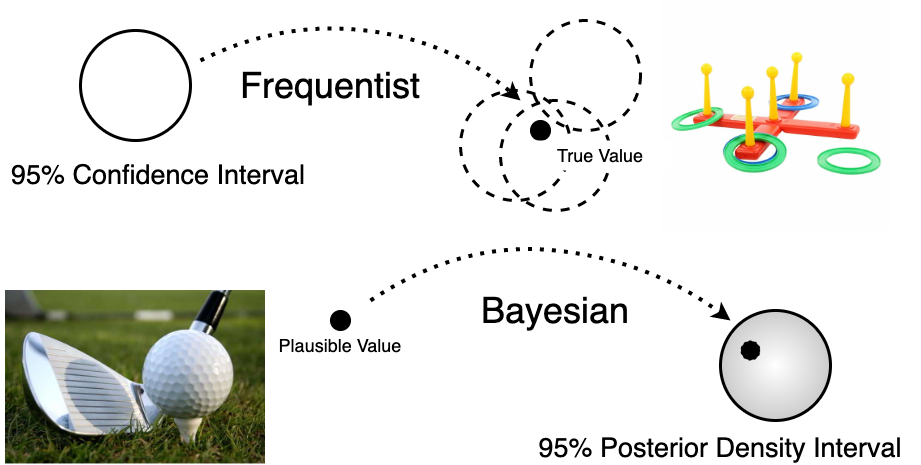
\includegraphics[width=0.8\linewidth]{img/confidence-intervals}
\end{figure}
\begin{block}{Suggested Reading}
\href{https://evolution.gs.washington.edu/gs560/2011/lecture3.pdf}{Explanation of P-values} by Joe Felsenstein
\end{block}
\end{frame}
\begin{frame}{Hypothesis Testing in H0, H1 framework}
    You should know what is hypothesis testing, t-test, p-values.
    \begin{itemize}
        \item 1 sample mean test ${\displaystyle t={\frac {Z}{s}}={\frac {{\bar {X}}-\mu }{{\widehat {\sigma }}/{\sqrt {n}}}}}$
        \item 2 sample mean test ${\displaystyle t={\frac {{\bar {X}}_{1}-{\bar {X}}_{2}}{s_{p}{\sqrt {\frac {2}{n}}}}}},\quad{\displaystyle s_{p}={\sqrt {\frac {s_{X_{1}}^{2}+s_{X_{2}}^{2}}{2}}}}, ...$
        \item 2 sample not equal variances, now equal sample sizes test $...,{\displaystyle s_{p}={\sqrt {\frac {\left(n_{1}-1\right)s_{X_{1}}^{2}+\left(n_{2}-1\right)s_{X_{2}}^{2}}{n_{1}+n_{2}-2}}}}$
    \end{itemize}
    \begin{block}{Too Complicated}
    The less assumptions we have, the more complicated is math and implementation
    \end{block}
\end{frame}
\section{Hypothesis Testing}
\begin{frame}{Bayesian Tools}
    \begin{enumerate}
        \item Highest Density Interval
        \item Region of Practical Equivalence
        \item Bayes Factor
        \item Custom
    \end{enumerate}
\end{frame}
\subsection{Highest density interval}
\begin{frame}{Highest Density Interval}
    \begin{columns}
    \begin{column}{0.5\linewidth}
    HDI The most popular way to interpret the posterior
    \begin{enumerate}
        \item Represents a range of most probable values
        \item Easy to interpret and calculate
        \item Easy to visualize
    \end{enumerate}
    \begin{block}{Example}
    \begin{itemize}
        \item With 95\% probability effect size in range [A, B]
        \item Range [A, B] represents 95\% of most probable effect sizes
    \end{itemize}
    \end{block}
    \end{column}
    \begin{column}{0.5\linewidth}
    \begin{figure}
        \centering
        \includegraphics[width=\linewidth]{img/hdi}
        \caption{Highest Density Interval}
    \end{figure}
    \end{column}
    \end{columns}
\end{frame}
\subsection{Region of Practical Equivalence}
\begin{frame}{Region of Practical Equivalence}
\begin{columns}
\begin{column}{0.5\linewidth}
RoPE is a common way to say if a parameter estimate is "significant". The use case:
\begin{enumerate}
    \item You do not care if the effect size is less than $0.1$
    \item Plot the region overlapping with the posterior
    \item Decide
\end{enumerate}
\begin{block}{Example}
    The effect size "E" is out of the region of practical equivalence so we treat it as a significant one
\end{block}
\end{column}
\begin{column}{0.5\linewidth}
\begin{figure}
    \centering
    \includegraphics[width=\linewidth]{img/rope}
    \caption{Rope Plot}
\end{figure}
\end{column}
\end{columns}
\end{frame}
\begin{frame}{Bayes Factor}
\begin{columns}
    \begin{column}{0.5\linewidth}
    IMO the most complicated to explain statistic.
    \begin{enumerate}
        \item Similar to the Frequentist p-value
        \item Harder to interpret and explain to people
        \item Checks H0 vs H1 for $x_0$
    \end{enumerate}
    \begin{block}{Definition}
        Bayes Factor is defined as the ratio of the likelihood of one particular hypothesis to the likelihood of another hypothesis
    \end{block}
    \end{column}
    \begin{column}{0.5\linewidth}
    \begin{figure}
        \centering
        \includegraphics[width=\linewidth]{img/bayes-factor}
        \caption{$\text{BF} = \frac{
        \textcolor{red}{\operatorname{pdf}_{H1}(x_0)}
        }{
        \textcolor{blue}{\operatorname{pdf}_{H0}(x_0)}
        }$}
        \label{fig:my_label}
    \end{figure}
    \end{column}
\end{columns}
\end{frame}
\subsection{Custom Hypothesis}
\begin{frame}{Custom Queries}
\begin{columns}
    \begin{column}{0.5\linewidth}
    You can do much more!
    \begin{enumerate}
        \item $P(A < 0)$
        \item $P(A > B)$
        \item $P(\max(A) > \max(B))$
        \item $P(A = \argmax(A, B, C, D))$
        \item $P(\text{profit}(X, \Theta) > \$100)$
        \item Quantiles - $Q_{0.05}(\text{profit}(X, \Theta))$
    \end{enumerate}
    \end{column}
     \begin{column}{0.5\linewidth}
    \begin{figure}
        \centering
        \includegraphics[width=\linewidth]{img/p_a_lt_0}
        \caption{$P(A<0)$}
    \end{figure}
    \end{column}
\end{columns}
    
\end{frame}
\subsection{}
\begin{frame}{Takeouts}
\begin{columns}
    \begin{column}{0.5\linewidth}
    Bayesians have a Swiss Knife for Hypothesis Checking
    \begin{enumerate}
        \item Numerous ways to interpret results
        \item Not a Yes/No answer
        \item Uncertainty is obviously represented
        \item Flexibility in analysis
        \item Easy to implement
        \item Easy to interpret
    \end{enumerate}
    \end{column}
    \begin{column}{0.5\linewidth}
    \begin{figure}
        \centering
        \includegraphics[width=\linewidth]{img/swiss-knife}
        \caption{Bayesian Hypothesis Testing}
    \end{figure}
    \end{column}
\end{columns}
\section{AB Testing}
\end{frame}
\begin{frame}{Types of Problems}
\begin{columns}
    \begin{column}{0.5\linewidth}
    Bayesian AB testing is widely applicable
    \begin{enumerate}
        \item<alert@2> Discrete Observations (views and clicks)
        \item<alert@2> Continuous Observations (read time, spent amount)
        \item<alert@3> With Context Predictors (CUPED\cite{cuped})
        \item<alert@3> With Hierarchies (Regions)
    \end{enumerate}
    \visible<3>{
    \begin{block}{The hard part}
    Most of the above methods are still in development
    \end{block}
    }
    \end{column}
    \begin{column}{0.5\linewidth}
    \centering \Huge \textcolor{red}{A}/\textcolor{blue}{B}
    \end{column}
\end{columns}
\end{frame}
\subsection{Priors}
\begin{frame}{Approaching Priors}
\begin{columns}
    \begin{column}{0.5\linewidth}
    \begin{block}{Uplift $\lambda$}
        Relative change to the baseline
    \end{block}
    When you start the experiment, don't you know anything about the set of possible outcomes?
    \end{column}
    \begin{column}{0.5\linewidth}
    \includegraphics[width=\linewidth]{img/lambda_prior}
    \end{column}
\end{columns}
\end{frame}
\begin{frame}{Setting priors for Uplift}
You are in the preparation to run an experiment B vs holdout A. You might be interested in increasing the mean of statistics (average bill)
\begin{itemize}
\pause
\item<+-> Do you expect after changes in B you have a 1000\% increase? Very sure No
\item<+-> Do you expect after changes in B you have a 100\% increase? Very sure No
\item<+-> Do you expect after changes in B you have a 10\% increase? Unlikely
\item<+-> Do you expect after changes in B you have a 3\% increase? Maybe
\item<+-> Do you expect after changes in B you have a 3\% decrease? Maybe
\item<+-> Do you expect after changes in B you have an X\% decrease? Your answer
\end{itemize}
\begin{alertblock}{Relative or Absolute change?}
    Make it clear if the change is relative or absolute!
\end{alertblock}
\end{frame}
\section{Example}
\subsection{Prior}
\begin{frame}{Binomial Model Example}
    \begin{columns}
    \begin{column}{0.5\linewidth}
    \begin{itemize}
        \item The example is binary Yes/No choice
        \item Observations follow the Bernoulli likelihood
    \end{itemize}
    \begin{align*}
        x^A_i & \sim \operatorname{Bernoulli}(p_A)\\
        x^B_i& \sim \operatorname{Bernoulli}(p_B)
    \end{align*}
    Do we have additional information?
    \visible<2->{
    \begin{itemize}
        \item Historical $\bar p$
        \item Expected improvement $\pm \bar \sigma \%$ (e.g. $\pm 0.01\%$)
    \end{itemize}
    }
    \end{column}
    \begin{column}{0.5\linewidth}
    \includegraphics[width=\linewidth]{img/ab_testing.jpeg}
    \end{column}
    \end{columns}
\end{frame}
\begin{frame}{Adding Additional Information}
    \begin{columns}
    \begin{column}{0.5\linewidth}
    We can parametrize Beta distribution in a special way
    \visible<2->{
    \begin{align*}
        X & \sim \operatorname{Beta}(\alpha, \beta)\\
        \mu &= \frac{\alpha}{\alpha + \beta}\\
        \sigma &= \frac{\alpha\beta}{(\alpha+\beta)^2(\alpha+\beta+1)}\\
        X &\sim \operatorname{Beta}(\mu, \sigma) \Rightarrow\\
        &\Rightarrow \begin{cases}
        \alpha &= \mu \kappa\\
        \beta &= (1-\mu)\kappa\\
        \text{where}& \kappa = \frac{\mu (1 - \mu)}{\sigma^2} - 1\\
        \end{cases}
    \end{align*}
    }
    \end{column}
    \begin{column}{0.5\linewidth}
    \includegraphics[width=\linewidth]{img/beta_param}
    \begin{align*}
        G &\in \{A, B\}\\
        x^G_i & \sim \operatorname{Bernoulli}(p_G)\\
        p_G &\sim \operatorname{Beta}(\alpha_G, \beta_G)\;s.t. \\
        \E p_G &= \bar p, \\
        \operatorname{Var} p_G &= \bar \sigma^2
    \end{align*}
    \end{column}
    \end{columns}
\end{frame}
\begin{frame}{Prior Specification}
\begin{columns}
\begin{column}{0.5\linewidth}
\begin{block}{Case Study}
Our historical levels of conversion are about 5\% (and fixed). We expect about 1\% \textbf{absolute} change ($\bar\sigma$) after implementing the solution. Or, similarly, 20\% \textbf{relative} change ($\bar\delta$).
\end{block}
\begin{align*}
    \bar p &= 0.05\\
    \bar \sigma &= 0.01 = \bar\delta \cdot 0.05\\
    G &\in \{A, B\}\\
    p_G &\sim \operatorname{Beta}(\mu=\bar p, \sigma=\bar\sigma)
\end{align*}
\end{column}
\begin{column}{0.5\linewidth}
\includegraphics[width=\linewidth]{img/beta_param_1}
\visible<2>{
\begin{block}{Takeout}
Special Beta parametrization leads to more interpretable priors
\end{block}
}
\end{column}
\end{columns}
\end{frame}
\subsection{Preparing an experiment}
\begin{frame}{Key questions be for you start}
\begin{columns}
\begin{column}{0.5\linewidth}
\begin{itemize}
        \item How much time can be allocated for the test?
        \begin{itemize}
            \item How accurate is the decision then?
        \end{itemize}
        \item How accurate should be the decision?
        \begin{itemize}
            \item How much time will be allocated for the test?
        \end{itemize}
    \end{itemize}
    \visible<2>{
    \begin{block}{Impossibility}
    You can't be fast in data collection and accurate at the same time
    \end{block}}
\end{column}
\begin{column}{0.5\linewidth}
\includegraphics[width=\linewidth]{img/fast_accurate}
\end{column}
\end{columns}
\end{frame}
\subsection{Parameter Recovery}
\begin{frame}{Parameter Recovery Study}
    Parameter recovery is a simulated experiment to know your model better. 
    \begin{enumerate}
        \item Generate data from a model configuration
        \item Pretend you do not know the true values
        \item Run inference for your model
        \item Compare estimated parameters and ground truth ones
    \end{enumerate}
    Given the results
    \begin{itemize}
        \item How well can you infer the model state?
        \item<alert@2> How does data size affects the results?
        \item Are there unidentifiable parameters? 
    \end{itemize}
    \begin{block}{Suggested Reading}
    Chapter 4 in \href{https://arxiv.org/abs/2011.01808}{Bayesian Workflow}
    \end{block}
\end{frame}
\begin{frame}{Parameter Recovery for AB testing}
\begin{columns}
\begin{column}{0.6\linewidth}
Given:
\begin{itemize}
    \item<1-> Effect is significant if $|p-\bar p|>\bar \sigma$
    \item<2-> Ignore effects $|p-\bar p|<\bar \sigma$
    \item<3-> How large should be N to decide if the effect is significant?
    \item<4-> $N=0$, $N=1000$, $N=100000$?
    \item<5-> What metric to use to evaluate detect effectiveness?
\end{itemize}
\visible<6>{
\begin{block}{Key observation}
Effect detection is a classification problem. E.g. \textcolor{red}{negative}, neutral, \textcolor{green}{positive} effects. We can use ROC-AUC for multiclass
\end{block}
}
\end{column}
\begin{column}{0.4\linewidth}
Recall the model
\begin{align*}
    i&\in 1\dots N\\
    x_i & \sim \operatorname{Bernoulli}(p)\\
    p &\sim \operatorname{Beta}(\mu=\bar\mu, \sigma=\bar\sigma)
\end{align*}
\end{column}
\end{columns}
\end{frame}
\begin{frame}{AB Testing as classification}
\begin{columns}
\begin{column}{0.6\linewidth}
Some definitions of our classification setup
\begin{enumerate}
    \item<2-> Target \alert<2>{$\hat p$}, used for \alert<3>{data generation}
    \item<3-> Labels
    \begin{itemize}
        \item "0" is $\hat p < \bar p - \bar \sigma$, negative
        \item "1" is $\bar p - \bar \sigma < \hat p < \bar p + \bar \sigma$, neutral
        \item "2" is $\hat p > \bar p + \bar \sigma$, positive
    \end{itemize}
    \item<4-> Predictions (probabilities using the posterior):
    \begin{itemize}
        \item<alert@4> $P(\text{p is negative} \cond X_{\alert<5>{1:N}})$
        \item<alert@4> $P(\text{p is neutral} \cond X_{\alert<5>{1:N}})$
        \item<alert@4> $P(\text{p is positive} \cond X_{\alert<5>{1:N}})$
    \end{itemize}
\end{enumerate}
\visible<5->{
\begin{block}{Run the simulation study}
\begin{enumerate}
    \item for $\hat p\in \dots$, for \alert<5>{$N\in \dots$} get $p(p\cond X_{\alert<5>{1:N}})$
    \item for \alert<5>{$N\in \dots$} calculate ROC-AUC
\end{enumerate}
\end{block}
}
\end{column}
\begin{column}{0.4\linewidth}
Recall the model
\begin{align*}
    i&\in \alert<5>{1\dots N}\\
    \alert<3>{x_i} & \alert<3>{\sim \operatorname{Bernoulli}(p)}\\
    \alert<2>{p} &\alert<2>{\sim \operatorname{Beta}(\mu=\bar\mu, \sigma=\bar\sigma)}
\end{align*}
\alert<4>{Posterior $p(p\cond X_{\alert<5>{1:N}})$}
\end{column}
\end{columns}
\end{frame}
\begin{frame}{ROC-AUC in Action}
    \begin{figure}
        \centering
        \includegraphics[width=\linewidth]{img/roc-auc}
        \caption{ROC-AUC increases as you get more data}
    \end{figure}
    \begin{columns}
    \begin{column}{0.5\linewidth}
    \textbf{Time is constraint:}
    \begin{enumerate}
        \item Discuss maximum affordable time
        \item Consult the plot for the expected ROC-AUC in decision
    \end{enumerate}
    \end{column}
    \begin{column}{0.5\linewidth}
    \textbf{ROC-AUC is constraint:}
    \begin{enumerate}
        \item Discuss minimum required ROC-AUC
        \item Consult the plot for the expected data size
    \end{enumerate}
    \end{column}
    \end{columns}
\end{frame}
\subsection{Posterior Simulations}
\begin{frame}{After the Inference}
\begin{columns}
\begin{column}{0.5\linewidth}
\textbf{Situation:} you've run the test for the aforehand specified duration. Key questions:
    \begin{enumerate}
        \item Which alternative to choose?
        \item What is the comparison criterion?
        \item Is the criterion connected to the real life?
    \end{enumerate}
    \visible<2>{
    \begin{block}{A better metric}
    A good metric is the one that is connected to expected profit.
    \end{block}
    }
\end{column}
\begin{column}{0.5\linewidth}
\begin{figure}
    \centering
    \includegraphics[width=\linewidth]{img/uplift_results_example}
    \caption{Example ROPE plot}
\end{figure}
\end{column}
\end{columns}
\end{frame}
\begin{frame}{Interpreting the Posterior}
    How can we calculate a better mectic?
    \begin{itemize}
        \item<2-> Connect the conversion rate $p_A$ or $p_B$ to the company size audience
        \item<3-> Use "Customer Value" as a proxy for money effect
    \end{itemize}
    It could look like this:
    \visible<4->{
    \begin{align*}
    &\text{Monetization}_A =\\ \text{(Per User Value)} \times &\text{(Num Users)} \times \alert<5>{\Delta p_A} - \text{(Implementation Cost)} 
    \end{align*}
    }
    \visible<5->{
    \begin{block}{Use the posterior}
    We can calculate $p(\text{Monetization}_A\cond X_A)$ out of $p(p_A\cond X_A)$
    \end{block}}
\end{frame}
\begin{frame}{Monetization Posterior}
\begin{equation*}\text{(Per User Value)} \times \text{(Num Users)} \times \Delta p_A - \text{(Implementation Cost)} 
    \end{equation*}
    \begin{columns}
    \begin{column}{0.4\linewidth}
    \begin{itemize}
        \item Implementation cost might differ
        \item Per User Value might have scenarios
        \begin{itemize}
            \item Positive
            \item Negative
            \item Average
        \end{itemize}
        \item You connect the experiment with business
        \item Compare outcomes with uncertainty
    \end{itemize}
    \end{column}
    \begin{column}{0.6\linewidth}
    \begin{figure}
        \centering
        \includegraphics[width=\linewidth]{img/monetization}
        \caption{$p(\text{Monetization}_G\cond X_G)$}
    \end{figure}
    \end{column}
    \end{columns}
\end{frame}
\section{}
\begin{frame}{Takeouts}
Real Life AB testing is full of challenges. Bayesian tools are still considered novel.
    \begin{enumerate}
        \item Framing the statistical test
        \begin{itemize}
            \item Setting priors
            \item Setting likelihood
        \end{itemize}
        \item Decision making before the test
        \begin{itemize}
            \item Parameter recovery study
        \end{itemize}
        \item Bayesian decision making
        \begin{itemize}
            \item Loss functions
            \item Scenario testing
        \end{itemize}
    \end{enumerate}
\end{frame}
\begin{frame}[allowframebreaks]
\frametitle{References}
\bibliographystyle{abbrv}
\bibliography{../../../references.bib}
\end{frame}
\end{document}
